\item Discoveries:
    \begin{itemize}
      \item Dimensionality reduction and graph theoretic approaches
        give different insights into the data and identify different
        patterns as being relevant to cognition (different peak
        orders).
        \item An insight common to both approaches is that high-order
          (greater than first order) dynamic correlations are
          informative about ongoing high-level cognitive processing.
          As the level of cognitive processing decreases, cognition is
          reflected by lower-order correlations.
        \item Correlations at different orders are also associated
          with different networks of brain regions.  However, which
          networks reflect which types of interactions depends on the
          current task.  In general, lower order correlations during
          auditory listening reflect processing of low-level
          (auditory) features; mid-order correlations reflect speech
          and linguistic processing; higher-order correlations reflect
          across-sensory integration (e.g. ties to visual areas) and
          cognitive control areas.  This hierarchy dissolves during
          lower-order cognitive processing.
      \end{itemize}


      %%%%%%%
      



Based on prior work ~\citep{DemeEtal19} and following the direction of the field ~\citep{Turk13} we think our thoughts might be encoded in
dynamic network patterns, and possibly higher order network
patterns (Fig.~\ref{fig:direction_of_field}). We sought to test this hypothesis by developing an approach
to inferring high-order network dynamics from timeseries data. 

One challenge in studying dynamic interactions is the
computational resources required to calculate higher-order correlations. 
We developed a computationally tractable model of network dynamics (Fig.~\ref{fig:methods}) that takes in a feature
timeseries and outputs approximated first-order dynamics (i.e.,
dynamic functional correlations), second-order dynamics
(reflecting homologous networks that dynamically form and disperse),
and higher-order network dynamics (up to tenth-order dynamic
correlations).

We first validated our model using synthetic data, and explored how
recovery varied with different underlying data structures and kernels.   We then 
applied the approach to an fMRI dataset
~\citep{SimoEtal16} in which participants listened to an audio
recording of a story, as well as scrambled versions of the same story
(where the scrambling was applied at different temporal scales).  We
trained classifiers to take the output of the model and decode the
timepoint in the story (or scrambled story) that the participants were
listening to. We found that, during the intact listening condition in the
experiment, classifiers that incorporated higher-order correlations
yielded consistently higher accuracy than classifiers trained only on
lower-order patterns (Fig.~\ref{fig:decoding_level},  a.\&d.).  By contrast, these
higher-order correlations were not necessary to support decoding the other
listening conditions and (minimally
above chance) during a control rest condition.  This suggests
that the cognitive processing that supported the most cogntively rich listening conditions
involved second-order (or higher) network dynamics.

Although we found decoding accuracy was best when incorporating
higher-order network dynamics for all but rest
  condition, it is unclear if this is a product of the brain or the
  data collection technique.  It could be that the brain is
  second-order or it could be that fMRI can
  only reliably give second-order interactions. Exploring this method
  with other data collection technique will be important to
  disentangle this question.



  \subsection*{Concluding remarks}

How can we better understand how brain patterns change over
time? How can we quantify the potential network dynamics that might be
driving these changes? One way to judge the techniques of the future is
to look at the trajectory of the fMRI field so far has taken so far
(Fig.~\ref{fig:methods}).  The field started with 
univariate activation, measuring the average activity for each voxel.
Analyses of multivariate activation followed, looking at spatial patterns of
activity over voxels. Next, correlations of activity were explored, first
with measures like resting connectivity that take temporal correlation
between a seed voxel and all other voxels then with full connectivty
that measure all pairwise correlations.  Additionally, this path of increasing
complexity also moved from static to dynamic measurements.  One
logical next step in this trajectory would be dynamic higher-order
correlations. We have created a method 
to support these calculations by scalably approximating dynamic higher-order
correlations.  







% finally, we sought to identify which specific brain areas were
% involved in supporting cognition through high-order interactions.
% we used the eigenvector centrality results, which preserves the
% original feature space when characterizing high-order dynamic
% correlations.  we found that first and second-order correlations
% reflected auditory and speech processing in all of the story
% listening conditions.  during intact story listening, third order
% correlations reflected integration with visual areas, and fourth
% order correlations recruited high-level cognition regions.  however,
% during listening to temporally scrambled stories, these higher-order
% correlations did not involve visual areas or high-order cognitive
% control regions.  during rest we found a much different set of
% patterns.  first order correlations involved counting networks; second-order
% correlations recruited visual networks; third-order correlations
% recruited working memory networks; fourth-order correlations
% recruited episodic memory areas.






\subsubsection*{Reverse inference}
The dynamic patterns we examine comprise high-dimensional correlation
patterns at each timepoint.  To help interpret the resulting patterns
in the context of other studies, we created summary maps by computing
the across-timepoint average pairwise correlations at each order of
analysis (first order, second order, etc., up to fifteenth order
correlations).  We selected the 10 strongest (absolute value)
correlations at each order.  Each correlation is between the dynamic
activity patterns (or patterns of dynamic high-order correlations)
measured at two RBF nodes (see \textit{Hierarchical Topographic Factor
  Analysis}).  Therefore, the 10 strongest correlations involved up to
20 RBF nodes.  Each RBF defines a spatial function whose activations
range from 0 to 1.  We thresholded each RBF at 0.999 to construct a
map of spherical components that denoted the endpoints of the 10
strongest correlations.  We then carried out a meta analysis using
Neurosynth~\citep{RubiEtal17} to identify the 10 terms most commonly
associated with the given map.  This resulted in a set of 10 terms
associated with the average dynamic correlation patterns at each
order.


%%%%
For each order $n \in \{1, 2, 3, 4}$
we used the selected kernel to compute the $(n-1)^\mathrm{th}$-order
DISFC timeseries across all participants (for $n = 1$ we simply
averaged the ``order 0'' activity timeseries across participants).  We
then computed the average $n^\mathrm{th}$-order correlations (over
time) by correlating the columns of the $(n-1)^\mathrm{th}$-order
DISFC timeseries.  This yielded a single $K$ by $K$
$n^\mathrm{th}$-order correlation matrix.  Separately for each
experimental condition and order of correlations, we identified the
endpoints of the 10 strongest (absolute value) correlations
(Fig.~\ref{fig:neurosynth}).




We used this kernel to compute 
%%%%


% we used temporal decoders to identify cognitivly relevant neural
% patterns in fMRI data (see forward inference section of methods).
% we explored two approaches to effiently computing high-order
% correlations: PCA (dimensionality reduction) and eigenvector
% centrality (graph measure).  both approaches yielded qualitatively
% similar results for the story listening conditions: intact story was
% best decoded using high-order correlations, whereas scrambled
% stories were best decoded using lower-order correlations.  both
% approaches also yielded slightly above-chance decoding of resting state times
% (perhaps picking up on decreasing attention and/or increasing
% mind-wandering as the resting state scan progressed).  The PCA-based
% approach achieved the highest decoding accuracy using
% non-correlational (activation-based) data, whereas the eigenvector
% centrality approach identified second-order correlations as being
% most informative about resting state times.




We next evaluated if our model of high-order correlations in brain activity can capture cognitively relevant brain patterns. We performed a decoding analysis, using cross validation to estimate (using other participants’ data) which parts of the story each weighted-mixture of higher-order brain activity pattern corresponded to (see \textit{Materials and methods}). We note that our primary goal was not to achieve perfect decoding accuracy, but rather to use decoding accuracy as a benchmark for assessing whether different neural features specifically capture cognitively relevant brain patterns.

Separately for each experimental condition, we divided participants
into two groups. For the zeroth order, we computed the mean factor
activity for each group.  For all subsequent orders up to the tenth
order, we computed the mean approximated dynamic ISFC of factor
activity for each group (see \textit{Materials and methods}), and
combined in a weighted mixutre with all previous orders
(i.e. cross-validation for the second
order contained a weighted-mixture of zeroth, first, and second order
(Fig.~\ref{fig:decoding_level}, c.\&f.).  For
each order, we correlated the group 1 activity patterns with group 2
activity patterns.  We then subdivided the group 1 to obtain an
optimal weighting parameter for each order’s correlation matrix using
the same cross validation method. We used the optimal weighting
parameters to obtain a weighted-mixture (see \textit{Materials and methods}) of each order’s correlation
matrix. Using these correlations, we labeled the group 1 timepoints
using the group 2 timepoints with which they were most highly
correlated; we then computed the proportion of correctly labeled group
1 timepoints. (We also performed the symmetric analysis whereby we
labeled the group 2 timepoints using the group 1 timepoints as a
template.) We repeated this procedure 100 times (randomly re-assigning
participants to the two groups each time) to obtain a distribution of
decoding accuracies for each experimental condition. There were 272
timepoints for paragraph condition, 300 timepoints for intact and word
conditions, and 400 timepoints for rest condition,  so chance
performance on this decoding test is was $\frac{1}{272}$,
$\frac{1}{300}$, and $\frac{1}{400}$ respectively.
 
We repeated this process for each set of parameters, varying kernel
type and width, and averaged over the reduction technique used to
approximate the higher-order correlations (PCA Fig.~\ref{fig:decoding_level},  a.-c. and eigenvector
centrality Fig.~\ref{fig:decoding_level},  d.-f.).  Since there is no ground truth in these analyses, and we did not know
which parameters best capture the data, we instead report a robustness
search by averaging over the parameters and reporting which results
consistently showed up across all parameters.
\begin{figure}
  \centering
  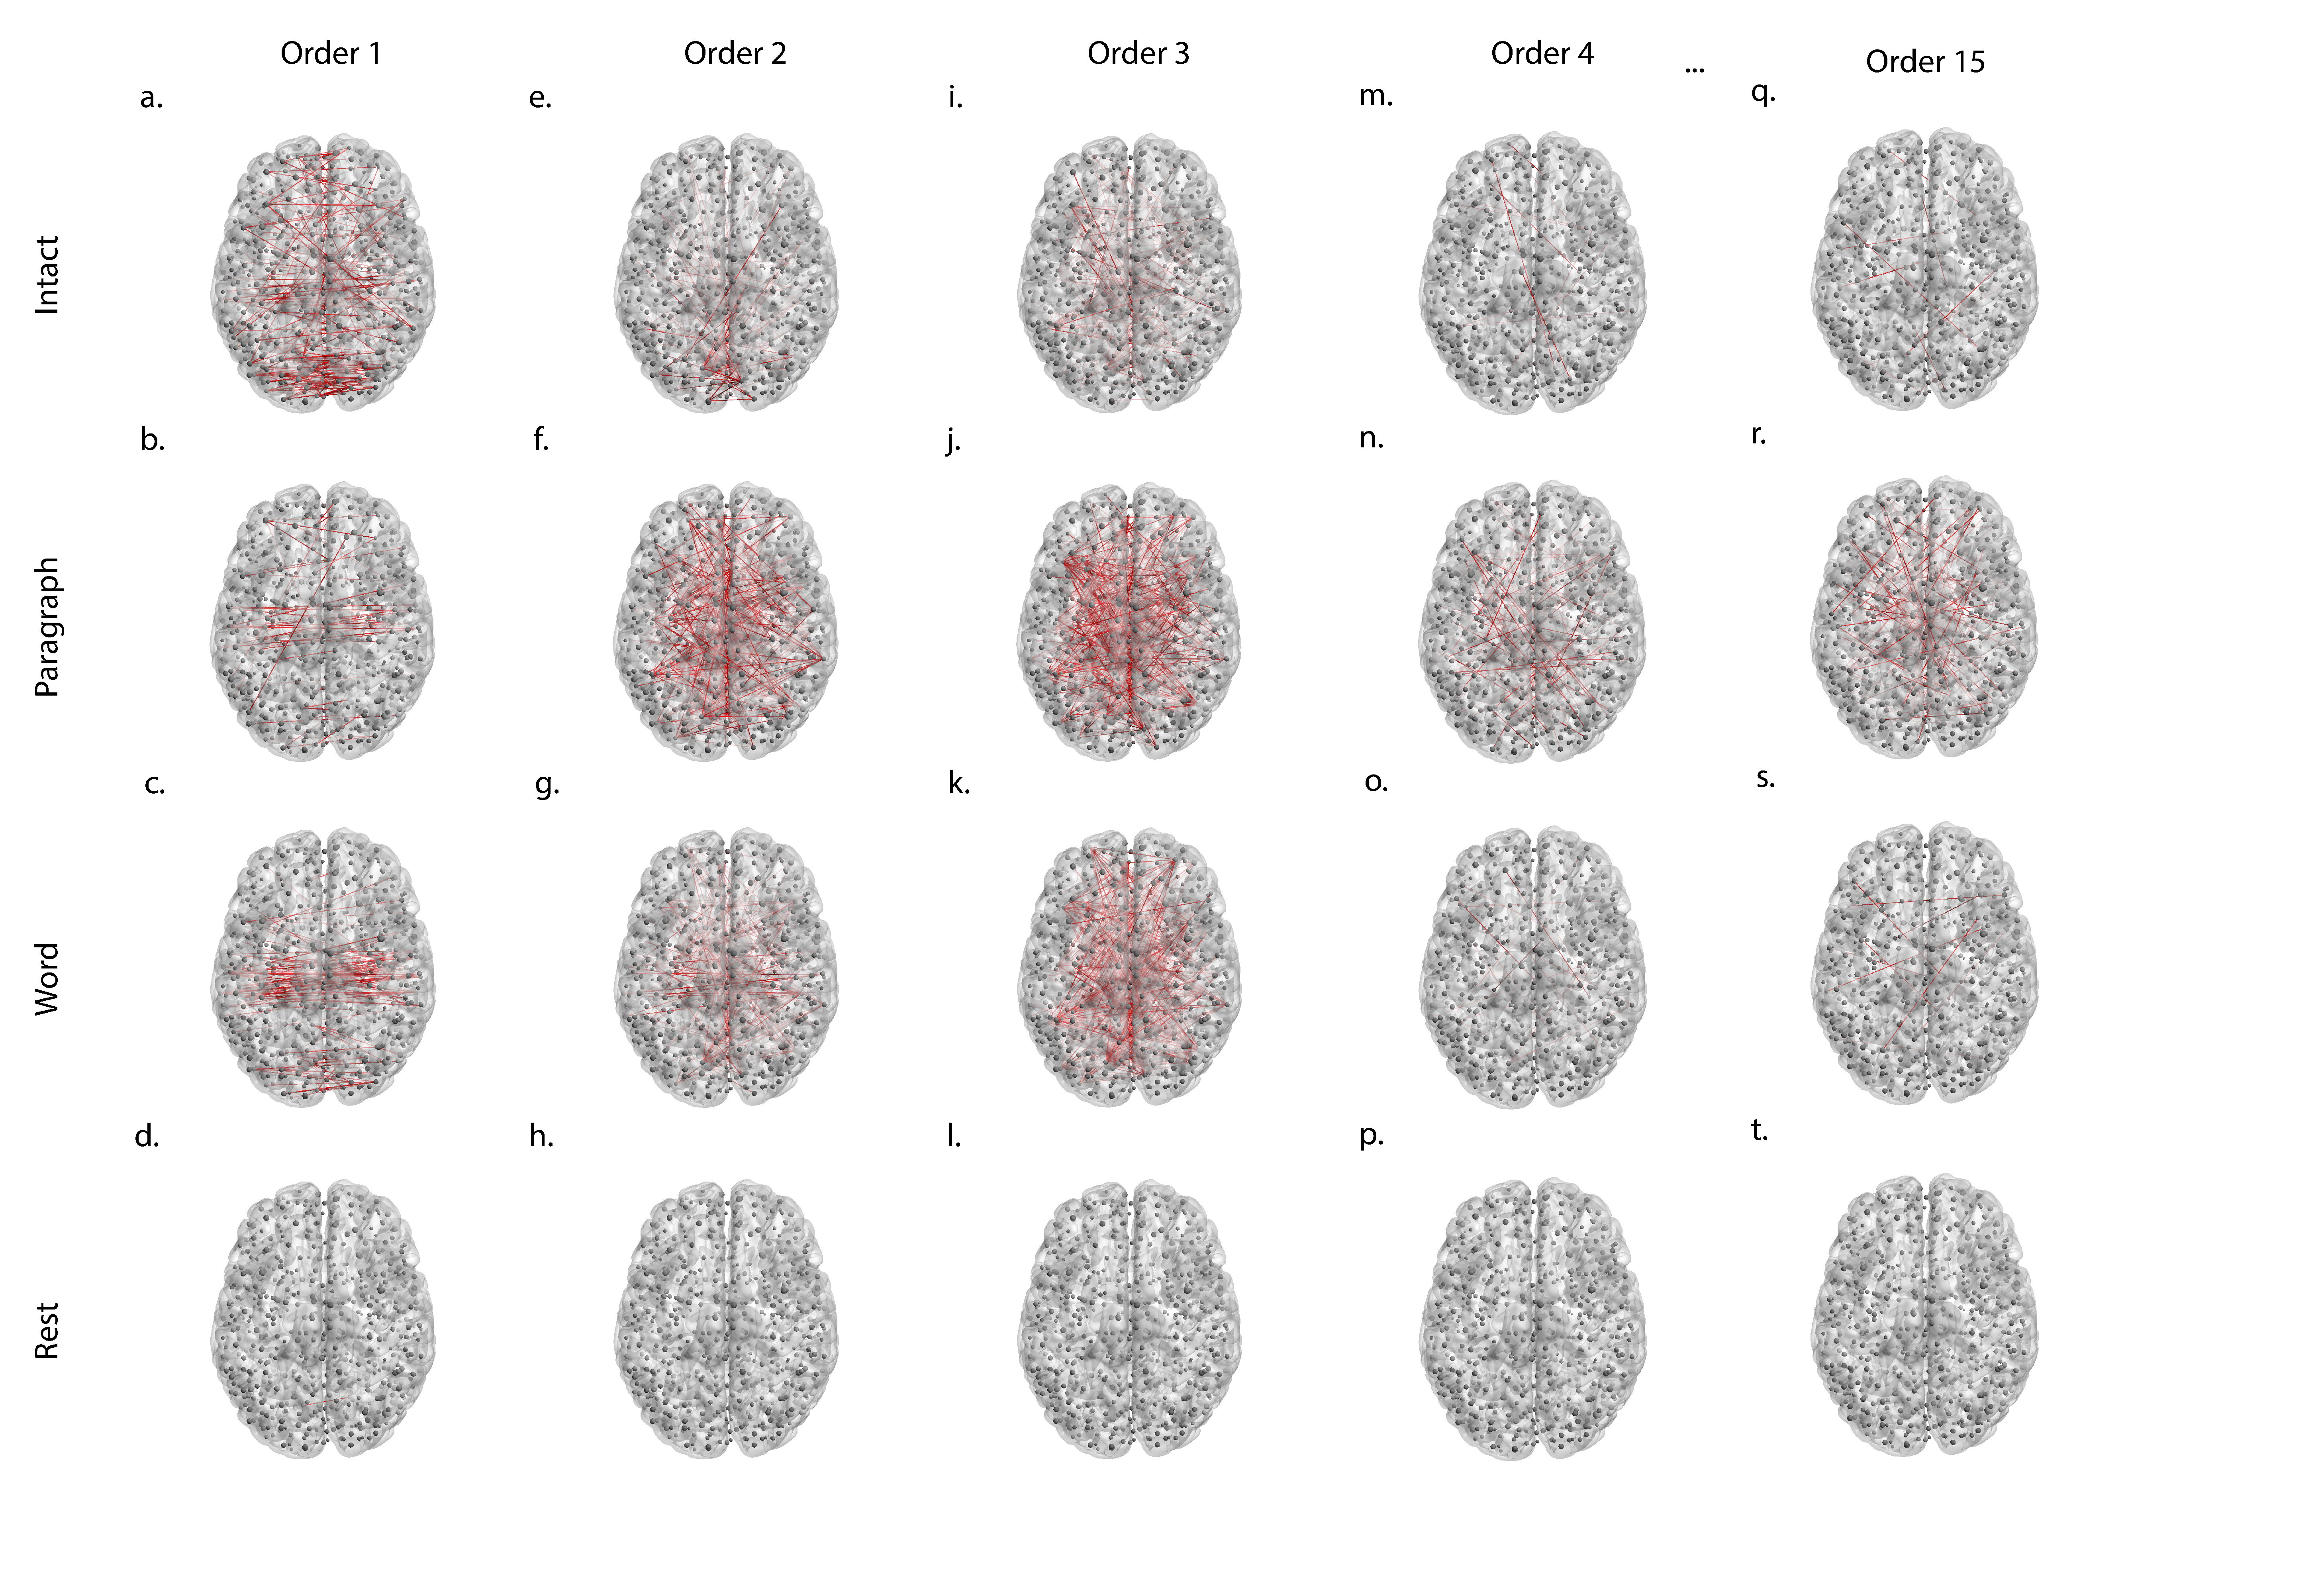
\includegraphics[width=\textwidth]{figs/brain_plots.pdf}
  \caption{\textbf{Average correlations by order for the intact listening condition.} Using eigenvector
    centrality to approximate higher-order correlations for the
    intact, paragraph scrambled, word scrambled, and rest condition.
    We plot the
    strongest 50\% absolute value
    mean correlation for \textbf{a.-d. first order, e.-h. second order,
      i.-l. third order, and m.-p. fourth order }, representing the degree of agreement by
    location pair over time.  To demonstrate how this method is
    computationally scalable, we also approximated
    \textbf{a.-d. fifteenth order} dynamic correlation, which would be
    possible to compute using conventional methods since it would require more bits to represent the solution than there are molecules in the universe.}
  \label{fig:brain_plots}
\end{figure}

The two methods used to approximate the higher-order correlations (PCA Fig.~\ref{fig:decoding_level},  a.-c. and eigenvector
centrality Fig.~\ref{fig:decoding_level},  d.-f.) capture different
facets of the activity patterns.  Using PCA, the higher-order
correlations are all linked to the original activity patterns, whereas
eigenvectory centrality breaks the immediate link with specific brain
areas and instead characterizes the position of the nodes in the
network that are similar over time.

We found for both PCA and eigenvector centrality, during the intact
condition in the experiment, classifiers that incorporated
higher-order correlations yielded consistently higher accuracy than
classifiers trained only on lower-order patterns
(Fig.~\ref{fig:decoding_level}, a.\&d.).  We plot the average
correlations for up to the fourth order for the intact condition
(Fig.~\ref{fig:brain_plots}) representing the degree of agreement by
location pair over time.  By contrast, we found that incorporating
higher-order (greater than first order) correlations did not further
improve decoding accuracy for the other listening conditions or rest
condition.  This suggests that the cognitive processing that supported
the most cognitively rich condition involved higher-order network
dynamics.



%synthetic data: we can recover dynamic correlations using different
%kernels
% wider kernels (Laplace, Gaussian) performed best when the
% correlations varied in a temporally structured way
% delta function kernels were best when the correlations varied
% randomly over time
% overall we recovered the structure we embedded in the data under all
% synthetic datasets we tested.  our approach performed best when the
% underlying correlational structure was either constant or gradually
% changing.  our approach performed worst when the underlying
% correlations varied randomly for one timepoint to the next.







\subsubsection*{Synthetic data}



To assess the performance of dynamic correlation recovery using
timecorr, we varied width the kernel and the specific structure of the
data. We applied timecorr, using delta and gaussian kernels
Fig.~\ref{fig:kernels}) to each of the following  
synthetic datasets: constant, random, ramping, and block.  We then correlated each recovered
correlation matrix with the ground truth. 

For the constant synthetic dataset, a gaussian kernel (width=10)
outperformed the delta kernel (Fig.~\ref{fig:synthetic_data},  a.).  This is in contrast with the random
synthetic dataset, for which the delta kernel best captures the
rapidly changing structure (Fig.~\ref{fig:synthetic_data},  b.). For
the ramping synthetic dataset, the slow changing strucutre within the
data is best
captured by the gaussian kernel and the best recovery occurs in the
middle (Ramping, Fig.~\ref{fig:synthetic_data},
c.). In addition to comparing the timecorr recovered correlation
matrices to the ground truth, we
further compared the ramping recovered correlation matrices to only the first random covariance matrix $K_{1}$
(First, Fig.~\ref{fig:synthetic_data},  c.) and to only the last
random covariance matrix $K_{2}$ (Last, Fig.~\ref{fig:synthetic_data},
c.), both of which perform best at the beginning and end respectively.

Similary for the block sythetic dataset, we compared the timecorr
recovered correlation matrices to the ground truth as well as to each
block-specific covariance matrix (Block 1-5,
Fig.~\ref{fig:synthetic_data},  d.).  Although the structure is
changing by block, the gaussian kernel once again outperforms the
delta kernel.  Performance does however drop near even boundaries for
when using the gaussian kernel.









For synthetic data where the true underyling dynamic correlations are
known, we are able to directly evaluate how well the recovered
correlations match the ground truth, for different choices of kernel
shape and width.  In contrast, or real-world data (where the ground
truth is not known), we use decoding accuracy to estimate whether a
given set of neural features reliably reflects ongoing stimulus-driven
cognitive processing.  However, under different circumstances,
different classifier properties (e.g., kernel shapes, kernel widths,
classification algorithm, etc.) will give rise to different decoding
accuracies.  We can average over different cross validation group
assignments to improve the stability of the decoding accuracy
assessments (to factor out effects due to particular group
assignments), but 

cannot know whether a given 


Because decoding accuracy is an indirect
reflection of how much a given set of neural features 

We cannot know which choice of kernel most accurately
reflects the ``true'' information content of the data.

For example, a
given kernel might highlight particular temporal aspects of the data
in a way that enhances or diminishes decoding performance.
\textbf{JRM STOPPED HERE}


\subsubsection*{Timepoint decoding}

Prior work has shown participants share similar neural responses to
richly structured stimuli when compared to stimuli with less
structure.  To assess whether the moment-by-moment higher order
correlations were reliably preserved across participants, we used
inter-subject functional connectivity (ISFC) to isolate the
time-varying correlational structure (functional connectivity patterns
that were specifically driven by the story participants listened to.
Following the analyses conducted by (HTFA)~\cite{MannEtal18}, we first
applied \textit{hierarchical topographic factor analysis} (HTFA) to
the fMRI datasets to obtain a time series of 700 node activities for
every participant.  We then computed the dynamic weighted ISFC using a
range of kernels and widths.  Specifically, we used Gaussian, Laplace,
and mexican hat kernels, as well as widths of 5, 10, 20, and 50.  We
then approximated these dynamic correlation using two reduction measures, PCA and eigenvector centrality, and computed the dynamic weighted ISFC on the approximations.  We repeated this process up to 10th order approximated correlations.  

To assess decoding accuracy, we randomly divided participants for each
stimulus into training and testing groups. For the zeroth order, we
computed the mean factor activity for each group.  For all subsequent
orders up to the tenth order, we computed the mean approximated
dynamic ISFC of factor activity for each group. To assess how
additional higher-order correlations contribute to decoding accuracy,
for each order we included a weighted-mixutre (described below) of the activity patterns of all
previous orders.  For each group of participants in turn, we compared these activity patterns (using Pearson correlations) to estimate the story times each pattern corresponded to. Specifically, we asked, for each timepoint: what are the correlations
between the first group's and second group's activity patterns at each
order. We note that the decoding test we used is a conservative in which we count a timepoint label as incorrect if it is not an exact match.

For each order we obtained the weighted-mixture of the correlation
matrices for the current order and all previous orders using mixing parameter, $\phi$, where $0 <\phi< 1$ reflects a
weighted mixture of order based decoding Fig.~\ref{fig:decoding_level}
Panel c. ). We calculated  $\phi$, by
subdividing the training group and using the quasi-Newton method of
Broyden, Fletcher, Goldfarb, and Shanno (BFGS ~\citep{NoceWrig06}) for optimization. We
repeated this cross-validation process 10 times for each parameter set. 














\subsection*{Evaluation metrics}
We evaluate our approach to extracting dynamic correlations and
higher-order correlations using several metrics detailed next.  First,
we generated synthetic data using known time-varying correlations, and
then we evaluated the fidelity with which Equation~\ref{eqn:timecorr}
could recover those correlations (for synthetic datasets with
different properties, and using different kernels to define the
weights; Fig.~\ref{fig:kernels}).  We then turned to a series of
analyses on a (real) neuroimaging dataset where the ground truth
correlations were \textit{not} known.  We evaluated whether the
recovered correlations could be used to accurately label held-out
neuroimaging data with the time at which it was collected.  We used this latter evaluations (using timepoint
decoding) as a proxy for
gauging how much explanatory power the recovered correlations held
with respect to the observed data.

\subsubsection*{Generating synthetic data}
To explore recovery of a constant covariance (Fig.~\ref{fig:synthetic_data},  a.), we generated syntheic
data sampled from a constant covariance matrix. To do this, we created one random
covariance matrix, $K$, with 50 features, and for each of the 300 timepoints  we
sampled from a Gaussian distribution centered on $K$.  Similarly, we generated synthetic data
sampled from a random covariance matrix (Fig.~\ref{fig:synthetic_data}, b.) by creating a new random
covariance matrix $K(t)$, for each of the 300 timepoints and sampled from a
Gaussian distribution centered on $K(t)$.

To generate synthetic data from a dynamically changing covariance
matrix (Fig.~\ref{fig:synthetic_data},  c.),
we generated two random covariance
matrices, $K_{1}$ and $K_{2}$.  We then computed a weighted average covariance matrix
for each of the 300 timepoint, $K(t)$, 
by taking the linearly spaced weights ($w$) of the two random matrices, 
\begin{align}
K(t) = w(t) * K_{1} + (1 - w(t)) *  K_{2}, \\\label{eqn:ramping}
\end{align}
and for each of the 300 timepoints sampled from a
Gaussian distribution centered on $K(t)$.

Lastly, for the synthetic data containing block structure (Fig.~\ref{fig:synthetic_data},  d.), we followed the same
process of creating synthetic data sampled from a constant covariance
matrix (see above) but sampled from a new random covariance matrix
after 60 consecutive timepoints.  We then pieced the blocks together
to create a sythetic dataset with 300 total timepoints but drawn from
5 separate covariance matrices. 

\subsubsection*{Recovery of ground truth parameters from synthetic
  data}


We applied timecorr, using delta and gaussian (width = 10) kernels
Fig.~\ref{fig:kernels}) to each of these 
synthetic datasets, then correlated each recovered
correlation matrix with the ground truth.  We repeated this process 10
times and explored how recovery varies
with the kernel and the specific structure of the data. For the
ramping synthetic dataset (Fig.~\ref{fig:synthetic_data},  c.)  and for the
block synthetic dataset (Fig.~\ref{fig:synthetic_data},  d.)  we made further
comparisons of the timecorr recovered correlation matrices. We
compared the ramping recovered correlation matrices to only the first random covariance matrix $K_{1}$
(First, Fig.~\ref{fig:synthetic_data},  c.) and to only the last
random covariance matrix $K_{2}$ (Last, Fig.~\ref{fig:synthetic_data},
c.) from Equation~\ref{eqn:ramping}. We also compared the block recovered correlation matrices in to
the block specific covariance matrix (Block 1-5,
Fig.~\ref{fig:synthetic_data},  d.).










A major challenge to studying such patterns is that typically neither
the correlations nor the hierarchical organizations of those
correlations may be directly observed.  Rather, these fundamental
properties must be inferred indirectly by examining the observable
parts of the system-- e.g., the behaviors of the individual units of
that system.  Here we propose a series of mathematical operations that may be used to approximate dynamic correlations at a range of scales (i.e., orders of interaction).

There are two basic steps to our approach (Fig.~\ref{fig:methods_fig}).  In the first step, we take
a number-of-timepoints ($T$) by number-of-features ($F$)
\textit{matrix of observations} ($\mathbf{X}$) and we return a $T$ by
$\frac{F^2 - F}{2}$ \textit{matrix of dynamic correlations}
($\mathbf{Y}$).  Here $\mathbf{Y_0}$ describes, at each moment, how
all of the features (columns of $\mathbf{X}$) are inferred to be
interacting.  (Since the interactions are assumed to be non-recurrent
and symmetric, only the upper triangle of the full correlation matrix
is computed.)  In the second step, we project $\mathbf{Y_0}$ onto an
$F$-dimensional space, resulting in a new $T$ by $F$ matrix
$\mathbf{Y_1}$.  Note that $\mathbf{Y_1}$ contains information about
the correlation dynamics present in $\mathbf{X}$, but represented in a
compressed number of dimensions.  By repeatedly applying these two
steps in sequence, we can examine and explore higher order dynamic
correlations in $\mathbf{X}$.

To understand the neuronal computations that support cognition, we
must understand the cooperative dynamics of populations of neurons.
These populations of neurons interact within each brain structure, and
the structures interact to form complex and dynamic networks. These
interactions, at each scale, vary according to the functions our
brains are carrying out and recent work has shown these dynamic
complex patterns support consciousness~\citep{DemeEtal19}.

In the last several decades, advances in functional magnetic resonance
image (fMRI) analyses have evolved to better characterize these
interactions of brain structures.  As~\cite{Turk13} outlines,
analyses using multivariate patterns of activity have given an advance
over univariate activity patterns because they allow relative
contributions of voxels to be combined and better assess distrubted
representations. Resting-state connectivity (RS) fMRI, which is the
temporal correlation of regions during rest, has shed light on the
rich and complex spatiotemporal organization of spontaneous brain
activity.  Functional connectivity (FC) has further characterized the
cognitive state dependency of this network organization.

Recent work has shown that FC fluctuates over time~\citep{ChanGlov10}~\citep[for review]{LuriEtal18}, and the assumed stationarity of these analyses may be too
simple to capture the dynamic nature of brain activity.  Additionally,
recent work has shown that temporal
variability in functional connectivity predicts attention task
performance~\citep{FongEtal19} and that
dynamic correlations between multivariate voxel patterns can add an
additional boost compared to static multivariate voxel patterns alone~\citep{MannEtal18}.




  
  Most complex systems reflect dynamic interactions between myriad
  evolving components (e.g., interacting molecules, interacting brain
  systems, interacting individuals within a social network or
  ecological system, coordinated components within a mechanical or
  digital device, etc.).  Despite that these interactions are central
  to the full system's behavior (e.g., removing a component from the
  full system can change the entire system's behavior), dynamic
  interactions cannot typically be directly measured.  Rather, the
  interactions must be inferred through their hypothesized role in
  guiding the dynamics of system components.  Here we use a
  model-based approach to inferring dynamic interactions from
  timeseries data.  In addition to examining first-order interactions
  (e.g., between pairs of components) we also examine higher-order
  interactions (e.g., that characterize mirrored structure in the
  patterns of interaction dynamics displayed by different subsets of
  components).  We apply our approach to two datasets.  First, we use
  a synthetic dataset, for which the underlying dynamic interactions
  are known, to show that our model recovers those ground-truth
  dynamic interactions.  We also apply our model to a neuroimaging
  dataset and show that the high-order dynamic interactions exhibited
  by brain data vary meaningfully as a function of the cognitive
  ``richness'' of the stimulus people are experiencing.



%should we introduce the name levelup in the introduction? ie. "in the second step, levelup, we use..." -ecw
%%%%%%%%%%%%%%%%%%%%%%%%
\section*{Methods}
%%%%%%%%%%%%%%%%%%%%%%%%

The mathematical theories behind the timecorr approach for calculating the moment-by-moment dynamic correlations in systems are described here. The function takes a number-of-timepoint by number-of-features matrix as well as a weight function to determine a moment-by-moment correlations matrix. To calculate the correlations, expectation values are found using equation 1: 

\begin{equation}
\mathrm{corr}_{x,y}(t) = \frac{1}{T} \sum_{t} \frac{\left(x(t)-\mathbb{E}[x]\right)\left(y(t)-\mathbb{E}[y]\right)}{\sigma_{x}(t)\sigma_{y}(t)}
\end{equation}

%should the variables in this equation/description change to match the description in the intro?
Here, x is the timepoint component of the matrix and y is the feature component. Timepoint by timepoint, x by x, at each given moment (t) in the matrix is subtracted from the expectation value of the full timepoint matrix. The same process occurs for the features points (y) at each timepoint (t). The product of these are then divided by the standard deviation at that moment for both the timepoint and the feature. Only the upper triangle of the matrix is calculated as the interactions are assumed to be both symmetric and non-recurrent. 

Two weight parameters have been used to calculate the connectivity of the data are a Gaussian weight parameter, equation 2, and a LaPlace weights parameter, equation 3. 

%label as Gaussian? 
\begin{equation}
\mathcal{N}\left( x | \mu, \sigma \right) = \frac{1}{\sqrt{2\pi\sigma^2}}\exp\left(-\frac{|| x - \mu ||^2}{2\sigma^2}\right)
\end{equation}
where sigma squared is the variance and mu is the expected value. 

%label as LaPlace? 
\begin{equation}
\mathcal{L}\left( x | \mu, \lambda \right) = \frac{1}{2 \lambda}\left( x | \mu, \lambda \right) = \exp\left(-\frac{|x - \mu|}{\lambda}\right)
\end{equation}
where mu is the expectation values, lambda is a defined decay constant. 

%figure showing the difference b/w two weights in same data set? Using the synthetic data?

When using the Gaussian weights parameter timepoints are more closely correlated to timepoints further away in the matrix than when using then the LaPlace weight function.

%Plot of kernels as Fig 1?

% New section? Mathematical Methods of Levelup? 
In order to understand how the data is interconnected we use the function levelup. Levelup uses the same input as the timecorr function, a timepoint-by-function matrix. 

%Diagram of input-->timecorr-->PCaA= levelup?

In the levelup method the the data first goes through the timecorr process and then is reduced using Principal Component Analysis (PCA). By utilizing PCA the output data maintains the same features as the input method. Not only does this allow for a sanity check, but also it allows for repeated use of the function. Using PCA or other reduction techniques is needed as without it the output data would get exponentially large. On the flip side using PCA, or any dimensionality reduction technique, makes the output data less accurate as information is lost. 


%PCA equation?
%figure/ chart of how many levels we "go up" before data gets too muddled- depends on the correlation?


Timepoints that share high similarity across all subjects have a high probability of being stimulus driven.

To compute the correlations of multiple subjects the across mode of both timecorr and levelup are used. The across function compares one voxel in a sample to the averages of that voxel in the rest of the dataframe. This occurs throughout every voxel in the dataset. The output of the across mode is a correlation matrix that is a number of timepoints by features matrix.

%F^2-F/2 +F 
